\section{Framework and overview}\label{sec:framework}

\subsection{testbed}
\note{describe machines and topology}

\subsection{consensus protocol}
\note{talk about consensus}

\subsection{Zookeeper}
\note{talk about basic operations here because they are mentioned in next subsection, talk also about modes of znode creation}.

\begin{figure}[h]
\centering
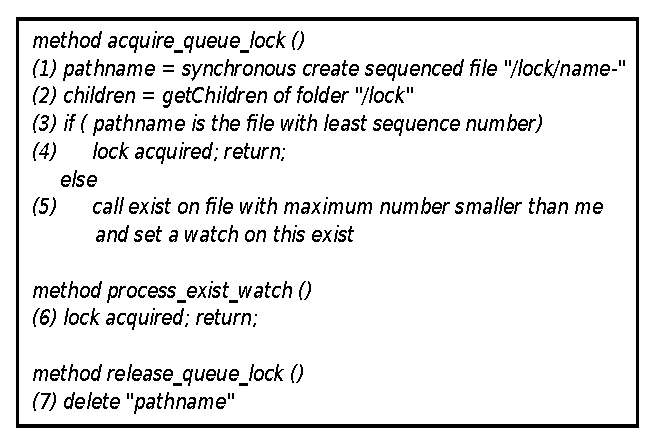
\includegraphics[scale=0.85]{img/queue_lock_pseudo.eps}
\caption{Pseudo code of acquiring and releasing queue locks}
\label{fig:queue_lock_pseudo}
\end{figure}

\subsection{synchronization primitives}

One of the main points studied in this paper is the effectiveness of synchronization primitives (primitives) and their comparative behavior giving different network conditions. Here we give a summary of the primitives we consider. Primitives are queue locks and test-and-set~(TAS). We divide primitives to synchronous and asynchronous depending on the client-server interactions. In the following we will summarize those primitives and how they translate in distributed systems using Zookeeper operations:
\begin{itemize}
\item{Synchronous queue lock: a queue structure maintaing the process of acquiring a lock. If a user tried to acquire a lock while another was holding it, then it is queued. Thus, users acquire the lock based on the order in which they entered the queue, helping achieve fairness. This is implemented in Zookeeper by synchronously creating an ephemeral, sequenced znode. Each create operation will return the file name, indicating the sequence number. The client waits until it has the smallest sequence number. Then, it acquire the lock. Releasing the lock is done by merely deleting the corresponding file. Pseudo code is displayed in Figure~\ref{fig:queue_lock_pseudo}. There are two possible execution paths. First, a user tries to acquire a lock while no one is holding it. In this case algorithm exist in line (4) after calling only two Zookeeper operations, namely synchronous \emph{create} and \emph{getChildren}. Second, another user is holding the lock when we try to acquire it. In this case the total latency is of operations \emph{creat}, \emph{getChildren}, and \emph{exists}, in addition to waiting time until the \emph{watch} returns to the client.}
\item{Synchronous TAS: to acquire a lock, the user repeatedly execute TAS until it succeeds. TAS tests a boolean flag until it flips it from false to true. Traditionally, TAS surfaced in memory-sharing systems due to the advent of atomic TAS operations. In Zookeeper we are able to create a primitive that is similar in spirit to hardware TAS. A user tries to create a file with a known name (all users try to create the same file). If the file already existed that means that another user is holding the lock and create will return an exception. Otherwise, the user will hold the lock. To release the lock, the user deletes the file. We repeatedly try to acquire a lock by calling \emph{create} in a busy loop. Alternatively, a watch on the file can be used to avoid busy waiting. Apparently, there is no order in entering the queue, hurting fairness. Execution path of TAS when no user is holding the lock is only one synchronous \emph{create} call. Otherwise, it is the time until the user is the fastest to create the file. A more detailed analysis of wait times are found in the analysis section. }
\item{Asynchronous primitives: }
\end{itemize}



